% F(AI)^2R conference poster, A0 portrait, three-column.
%
% This is the fifth primary artefact (paper, slides, poster, graph,
% logbook). The discipline of writing it forces the paper's spine
% to declare itself: what survives the cut is what is load-bearing.
%
% Build:    latexmk -pdf poster-A0.tex
% Output:   poster-A0.pdf  (A0 portrait, 841 x 1189 mm)
%
% Style: DLR Corporate Design --- Helvetica/Arial fallback,
% dlrBlau1 #00658B accent, mid-grey neutrals, square corners,
% hairline rules, no shadows / glows / gradients / 3D / emoji.
% Mirrors the colour ramps from paper/style/fair2r.sty so the
% poster renders the same as the paper's figures when held side
% by side.

\documentclass[25pt, a0paper, portrait, margin=20mm,
               innermargin=12mm, colspace=10mm,
               subcolspace=4mm, blockverticalspace=10mm]{tikzposter}

\tikzposterlatexaffectionproofoff

\usepackage[T1]{fontenc}
\usepackage[utf8]{inputenc}
\usepackage{amsmath}
\usepackage[scaled=1.0]{helvet}
\renewcommand{\familydefault}{\sfdefault}
\usepackage{microtype}
\usepackage{xcolor}
\usepackage{tikz}
\usetikzlibrary{arrows.meta, positioning, shapes.geometric, calc, fit}
\usepackage{graphicx}
% Resolve image references both when compiled in the slides/
% directory (CI: the build-slides workflow copies the paper PNGs
% into slides/ before compile) and when compiled standalone with
% the source tree intact (local: latexmk -pdf poster-A0.tex from
% slides/, with paper/figures/ as a sibling).
\graphicspath{{./}{../paper/figures/}{paper/figures/}}
\usepackage{enumitem}

% --- DLR colour ramps (mirror of paper/style/fair2r.sty) -------------
\definecolor{dlrBlau1}{HTML}{00658B}
\definecolor{dlrBlau2}{HTML}{3B98CB}
\definecolor{dlrBlau5}{HTML}{D1E8FA}
\definecolor{dlrGruen1}{HTML}{82A043}
\definecolor{dlrGruen5}{HTML}{E6EAAF}
\definecolor{dlrGelb1}{HTML}{D2AE3D}
\definecolor{dlrGelb5}{HTML}{FFF8BE}
\definecolor{dlrGrau1}{HTML}{666666}
\definecolor{dlrGrau3}{HTML}{B1B1B1}
\definecolor{dlrGrau4}{HTML}{CFCFCF}
\definecolor{dlrGrau5}{HTML}{EBEBEB}
\colorlet{dlrAccent}{dlrBlau1}
\colorlet{dlrAccentSoft}{dlrBlau5}

% --- Tikzposter theme: start from a clean built-in then override --
% the DLR palette through the existing colourlets. Custom themes
% in tikzposter print a debug stamp on the first page; we route
% around that by sticking with the built-in 'Simple' theme and
% overriding colours.
\usetheme{Simple}
\usecolorstyle{Default}
\colorlet{titlefgcolor}{dlrBlau1}
\colorlet{titlebgcolor}{white}
\colorlet{backgroundcolor}{white}
\colorlet{blocktitlefgcolor}{dlrBlau1}
\colorlet{blocktitlebgcolor}{dlrBlau5}
\colorlet{blockbodyfgcolor}{black}
\colorlet{blockbodybgcolor}{white}
\colorlet{framecolor}{dlrGrau1}

% Tighter line spacing for body text
\renewcommand{\baselinestretch}{1.05}

\title{\parbox{\linewidth}{\centering
       \color{dlrBlau1}\bfseries
       F(AI)\textsuperscript{2}R\\[2mm]
       \color{dlrGrau1}\mdseries\large
       FAIR Research with AI in the Loop, Twice}}
\author{\color{black}\bfseries Florian Krebs\\[1mm]
        \color{dlrGrau1}\mdseries
        ORCID 0000-0001-6033-801X \,$\cdot$\, florian.krebs@dlr.de\\[0.5mm]
        DLR Zentrum f\"ur Leichtbauproduktionstechnologie (ZLP), Augsburg}
\institute{\color{dlrGrau1}
           Helmholtz-Gemeinschaft \,$\cdot$\, NFDI4Ing \,$\cdot$\, HMC\\[1mm]
           \footnotesize\texttt{https://github.com/noheton/f-ai-r}}

\begin{document}
\maketitle[width=0.92\paperwidth, titletotopverticalspace=15mm]

% =============================================================
% LEFT COLUMN  --  the gap and why now
% =============================================================
\begin{columns}
\column{0.32}

\block{The gap}{
\textbf{FAIR was drafted for data}, then extended to research
software (FAIR4RS) and ML models (FAIR4ML). Neither extension
covers the artefacts \emph{LLM-assisted scholarly writing}
produces: transcripts, prompt files, model + tool version
manifests, verification-status ladders, per-claim provenance
maps. \textbf{If they vanish, the audit trail is gone}.
}

\block{Reported base rates}{
\centering\bfseries\color{dlrBlau1}\Large
\begin{tabular}{rl}
55\,\% / 18\,\% & GPT-3.5 / GPT-4 citation fabrication\\
                & \scriptsize\color{dlrGrau1}\mdseries
                  Walters \& Wilder, \textit{Sci.\ Rep.} 2023\\[1.5mm]
17--34\,\% & RAG-anchored legal hallucinations\\
                & \scriptsize\color{dlrGrau1}\mdseries
                  Magesh et al., Stanford RegLab 2024
\end{tabular}\\[3mm]
\color{black}\mdseries\normalsize
Detection alone is an arms race the reviewer side does not
win. An \textbf{authoring-side discipline} is the cheaper,
sturdier complement.
}

\block{Why now}{
The journal-as-distribution concept pre-dates the internet by
three centuries; preprint servers, overlay journals, and
artefact-versioned repositories now cover much of what
journals historically did. LLM-generated submissions on top of
a system already showing format strain tip a slow drift into a
visible crisis. F(AI)\textsuperscript{2}R is designed to fit
both the legacy and the emerging ecosystem.
}

% =============================================================
% CENTRE COLUMN  --  the position
% =============================================================
\column{0.36}

\block{The position}{
\centering
\large\color{dlrGrau1}\mdseries
The canonical FAIR axes with an \emph{(AI)} factor multiplied
through them, \textbf{squared}: each axis demands two passes
(authoring + audit), and (AI)\textsuperscript{2} unpacks into a
2$\times$2 of writer $\times$ reader.\\[2mm]
\normalsize\color{black}\mdseries
\begin{center}
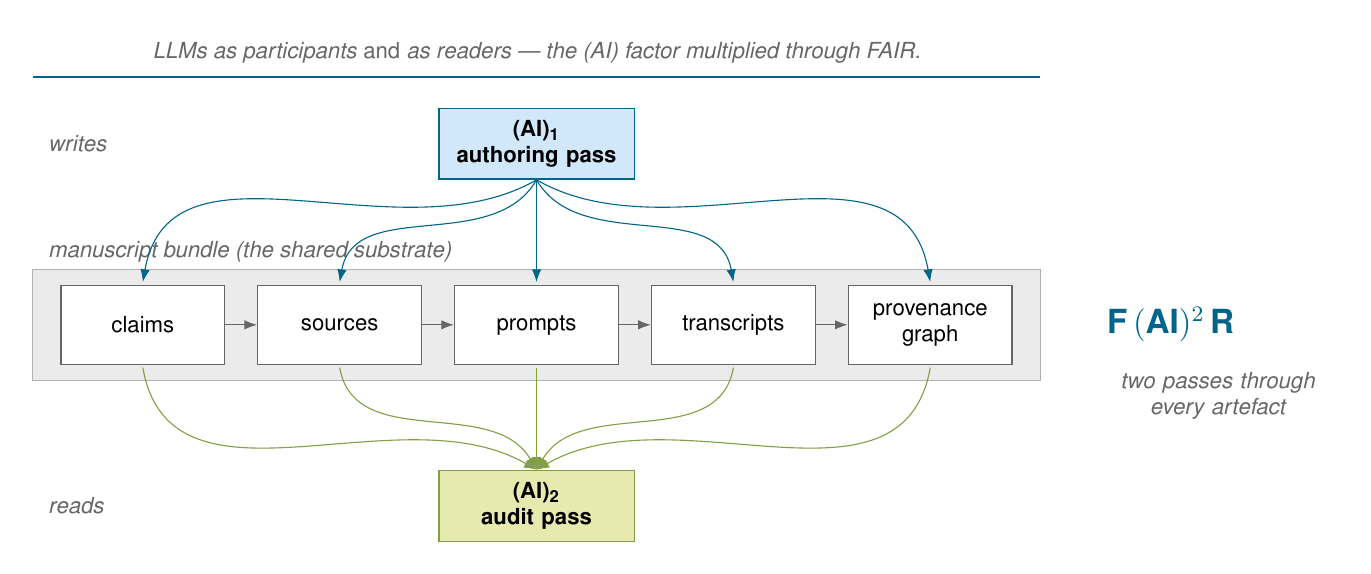
\includegraphics[width=0.95\linewidth]{hero.png}
\end{center}
\itshape Multiplicative, not appended. \emph{4AI hei{\ss}t alles}.
}

\block{Eight integrated practices}{
None individually novel; the integration is the contribution.
\begin{enumerate}[leftmargin=*, itemsep=2pt]
  \item Transcript preservation
  \item Verification-status labelling
  \item Per-claim provenance maps
  \item Mirror discipline (source / render)
  \item Recursive meta-process documentation
  \item Base-rate-anchored AI disclosure
  \item Legal honesty about authorship
  \item FAIR alignment as precondition
\end{enumerate}
\centering\itshape\color{dlrBlau1}
The pipeline is the team; the team is the methodology.\\
Specialisation reduces hallucination at the seam.
}

% =============================================================
% RIGHT COLUMN  --  the machinery and the live state
% =============================================================
\column{0.32}

\block{Verification ladder, live populations}{
\begin{center}
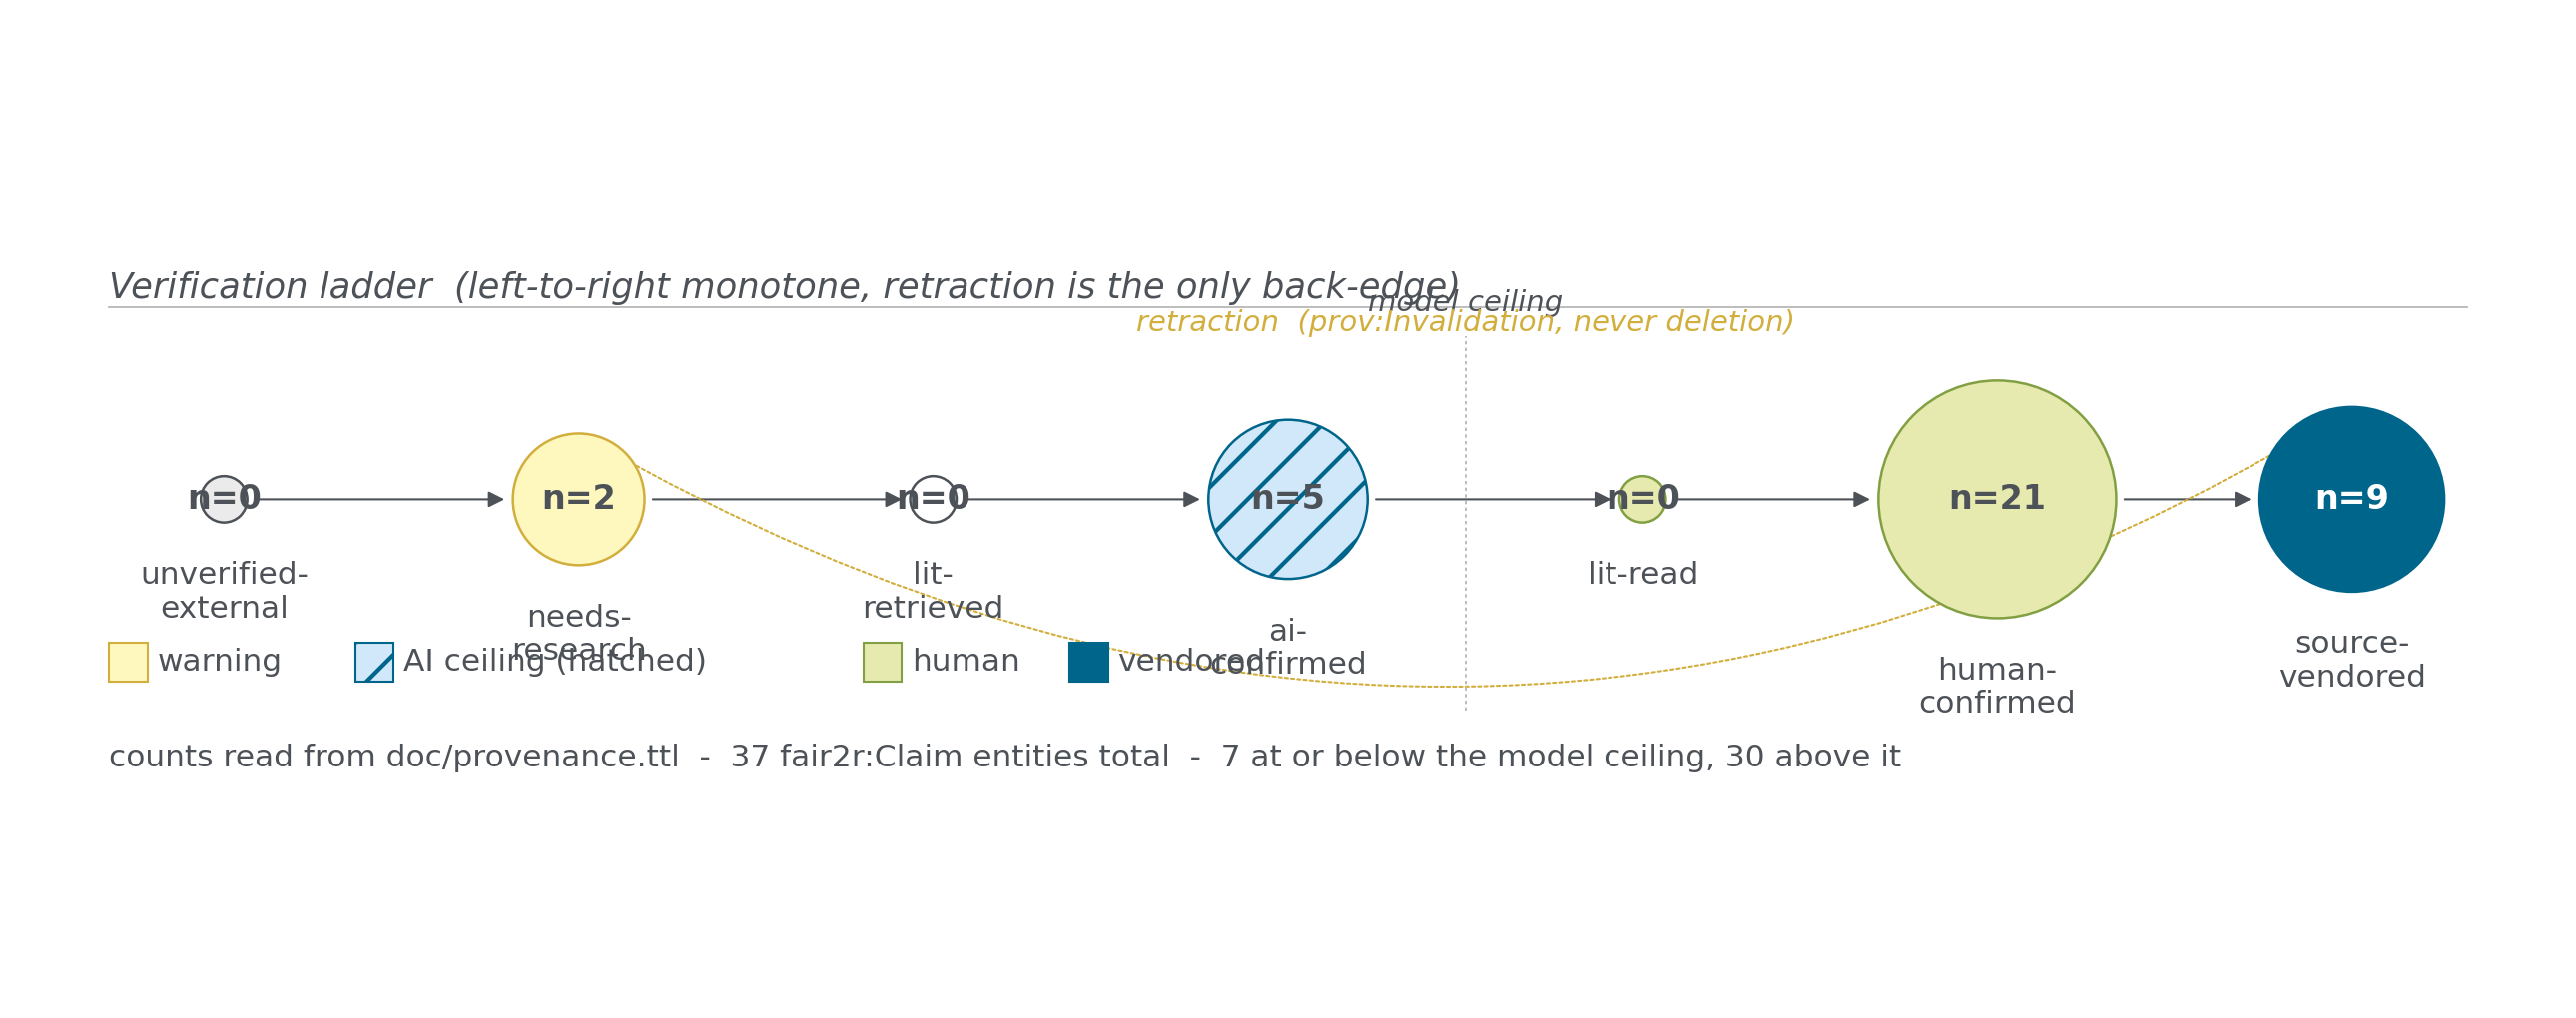
\includegraphics[width=0.96\linewidth]{ladder-populations.png}
\end{center}
A finite-state machine; node area $\propto$ count of
\texttt{fair2r:Claim} entities at that rung in
\texttt{doc/provenance.ttl}. The dotted rule is the
\textbf{model ceiling}: agent-deliverable rungs to the left,
human-only rungs to the right.
}

\block{Provenance graph as audit substrate}{
\begin{center}
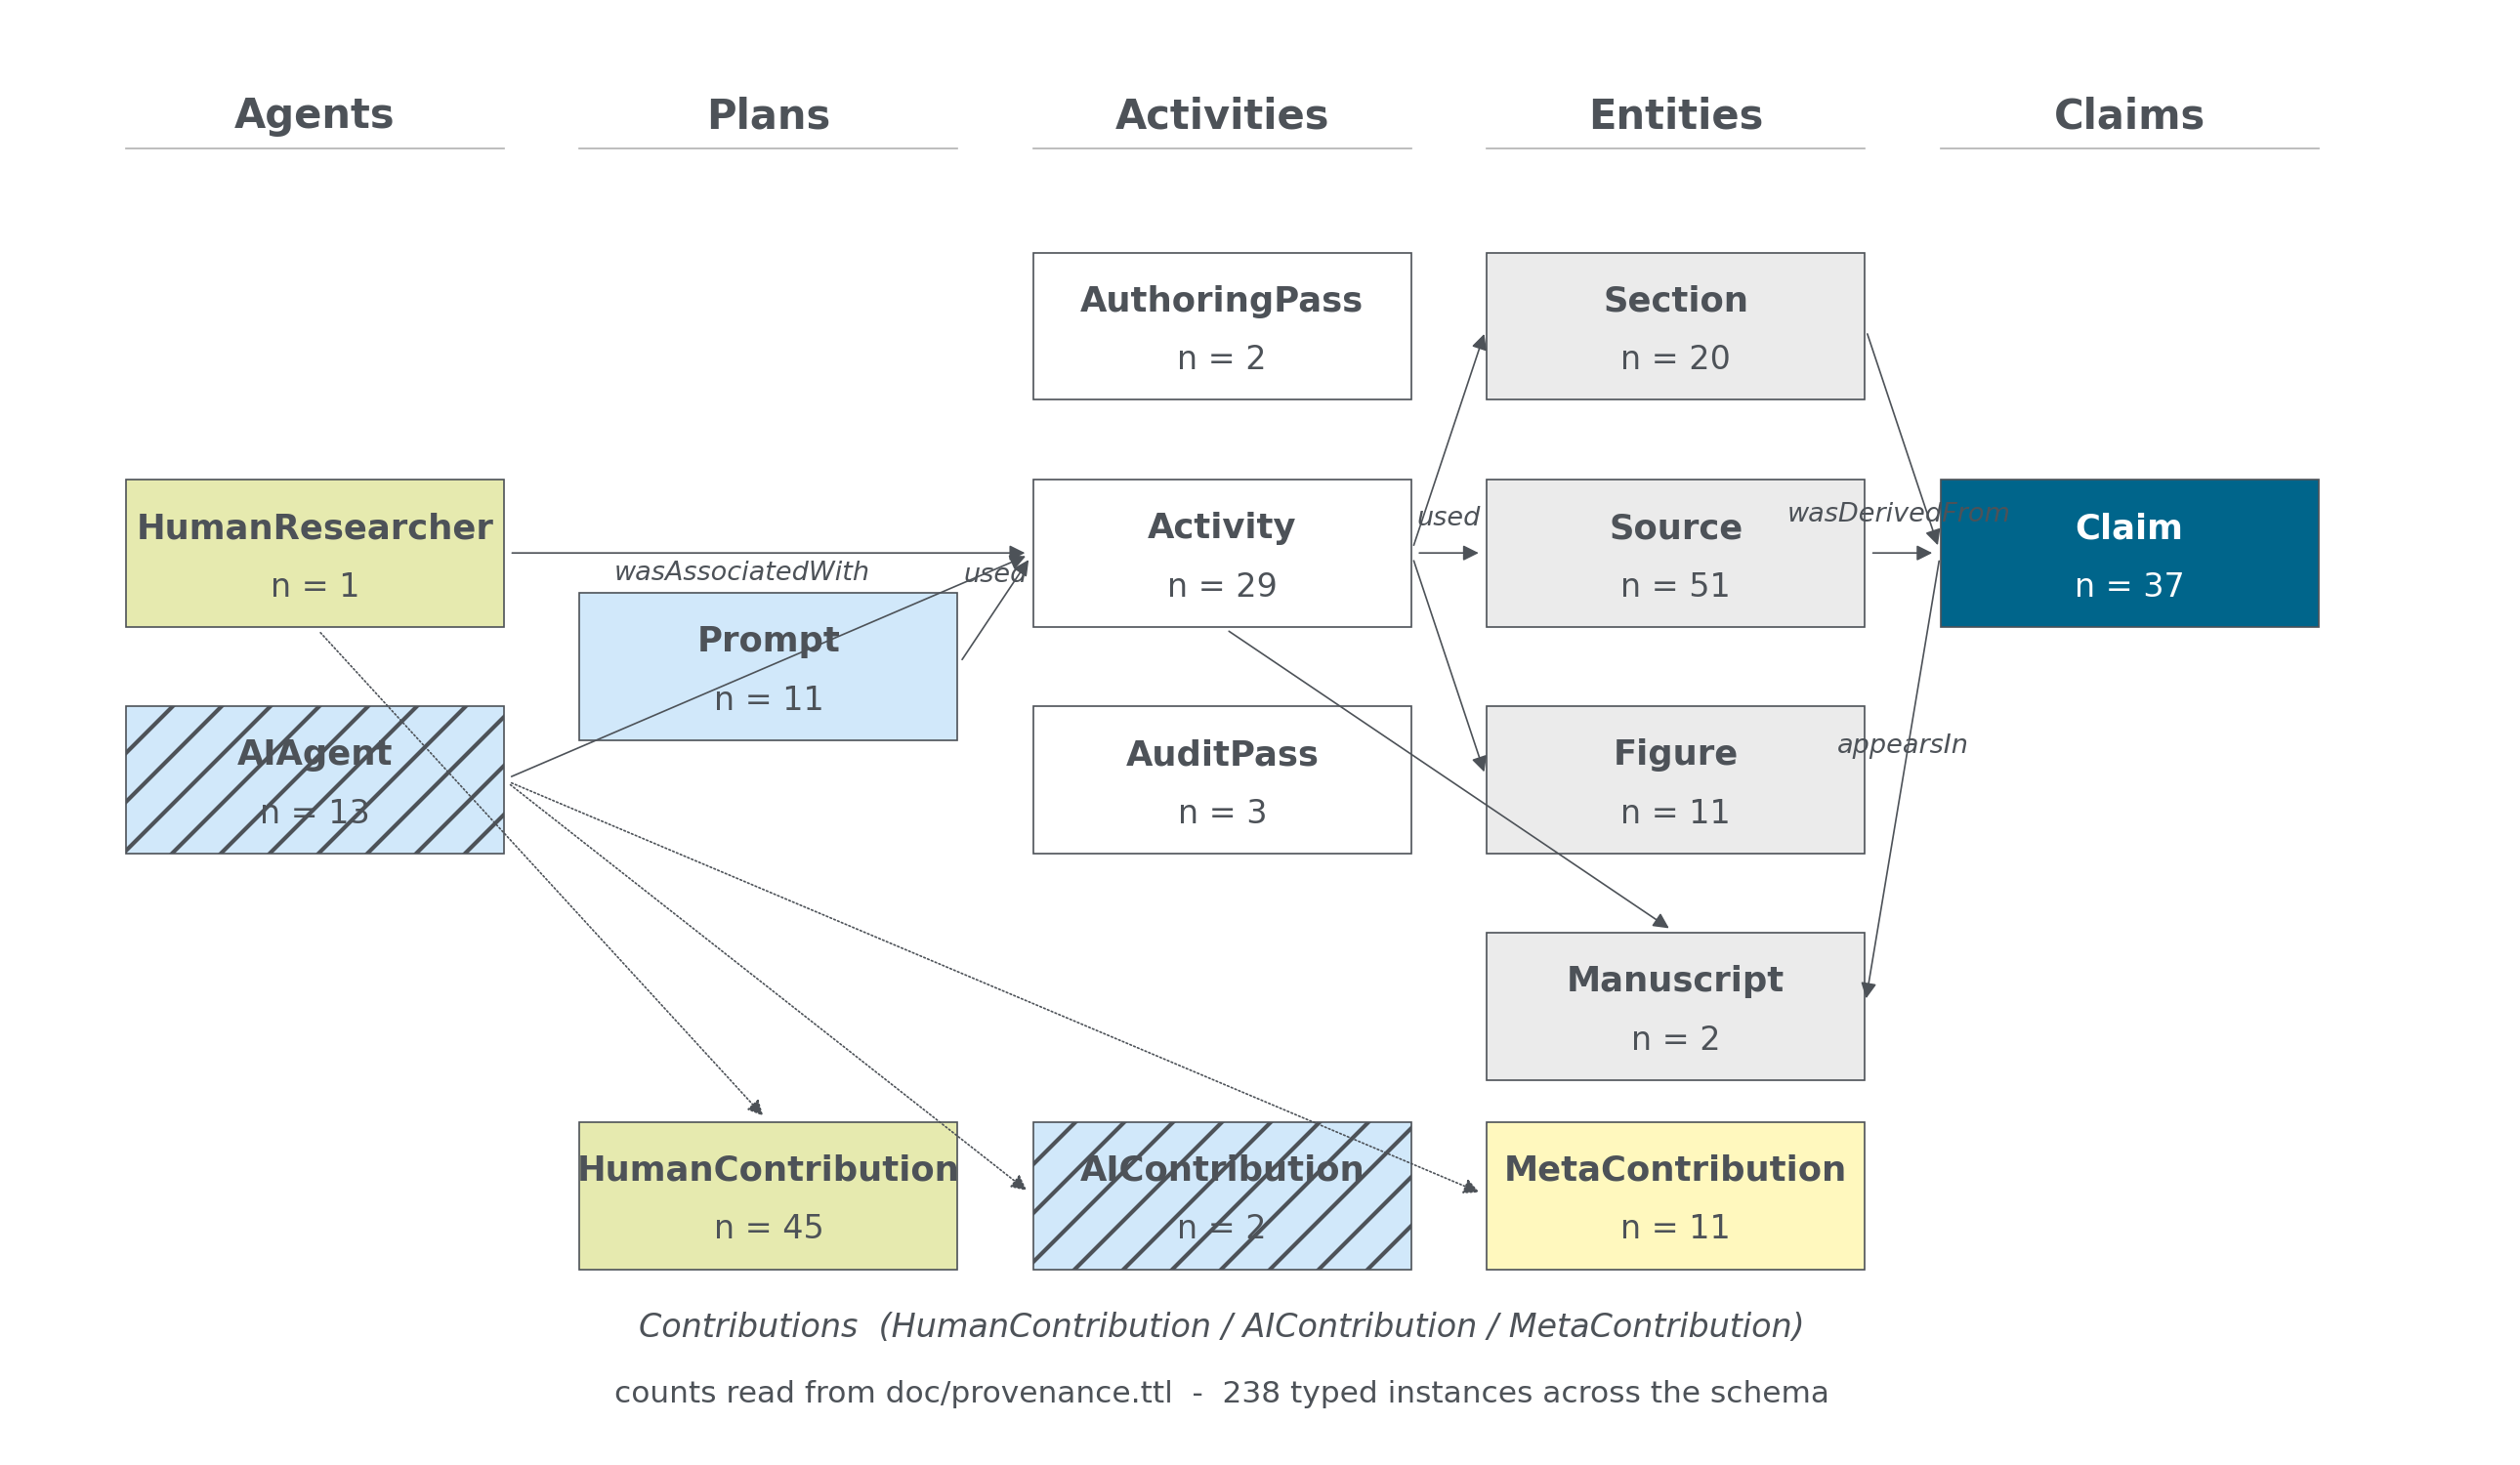
\includegraphics[width=0.96\linewidth]{provenance-topology.png}
\end{center}
Five PROV-O lanes plus a Contribution satellite band. Every
node carries its current instance count. \textbf{An audit run
is a SPARQL pass}, not a re-read.
}

\block{This is the worked example}{
\centering\normalsize\mdseries
This poster, the paper it summarises, the prompts, the
provenance graph, the logbook, and the build pipeline are all
in the public repository.\\[3mm]
\large\color{dlrBlau1}\bfseries
\texttt{github.com/noheton/f-ai-r}\\[1mm]
\large\color{dlrGrau1}\mdseries
\texttt{noheton.github.io/f-ai-r/}
}

\end{columns}

\node[anchor=south east, inner sep=8pt, font=\sffamily\scriptsize, color=dlrGrau1]
  at (current page.south east) {%
  Code: MIT \,$\cdot$\, Prose: CC-BY-4.0
  \,$\cdot$\, DRAFT --- not yet peer-reviewed%
};

\end{document}
